From the results of the various simulations, the percentage growth inhibition was calculated with respect to the control group two days after the end of the treatment as
$$ G.I. = 1 - \frac{A_t}{A_{nt}} $$ 
Where $A_t$ is the number of cancer cells in the treated group 48 hours after the end of the treatment and $A_{nt}$ is the number of cancer cells in the control at the same time. The values obtained are reportes in Table \ref{tab:gi}, alongside the values reported in the main paper and the ones obtained in the Cytarabine infusion condition.

\begin{table}[]
\begin{tabular}{|c|c|c|c|}
\hline
	Group & \begin{tabular}[c]{@{}c@{}}Growth \\ Inhibition (\%)\end{tabular} & GI (paper) & GI (exp) \\ \hline
Cyt low           & 11 & 10.0 & 9.0    \\ \hline
Cyt high          & 70 & 59.0 & 58.0   \\ \hline
Ibr low           & 44 & 43.4 & 43.5 \\ \hline
Ibr high          & 45 & 44.0 & 44.5 \\ \hline
Cyt + Ibr         & 96 & 95.0 & -    \\ \hline
Cyt infusion low  & 93 & -    & -    \\ \hline
Cyt infusion high & 98 & -    & -    \\ \hline
\end{tabular}
\caption{Growth inhibition calculated 2 days after the end of the treatments, with respect to the control group in the same day}
\label{tab:gi}
\end{table}

The discrepancy in the growth inhibition for the Cyt high group is probably due to some inconsistencies in the main paper, in which it is not clear when such value was calculated.

\begin{figure}[htbp!]
    \centering
    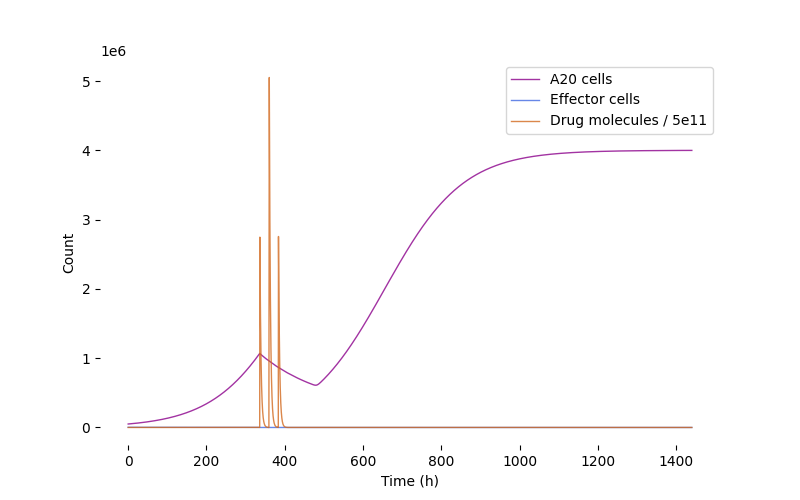
\includegraphics[scale = 0.45]{1-Cyt_high_2m.png}
    \caption{Simulation of the model with a high Cyt dose regimen}
    \label{fig:cyt-high}
\end{figure}

\begin{figure}[htbp!]
    \centering
    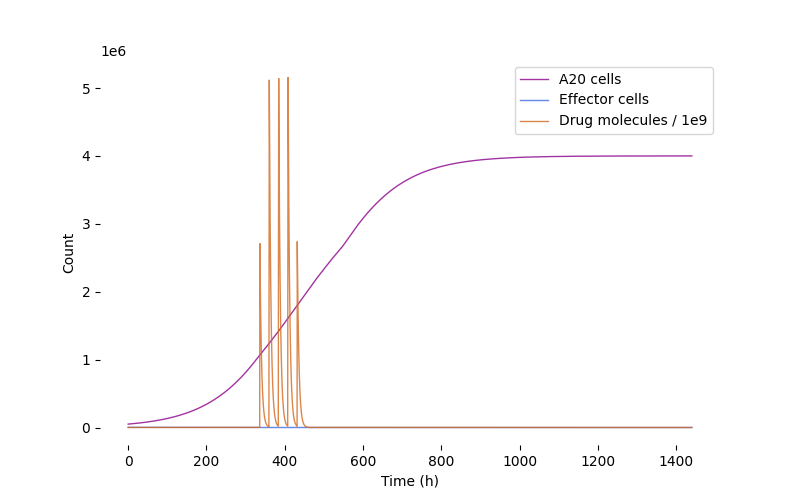
\includegraphics[scale = 0.45] {2-Cyt_low_2m.png}
    \caption{Simulation of the model with a low Cyt dose regimen}
    \label{fig:cyt-low}
\end{figure}

\begin{figure}[htbp!]
    \centering
    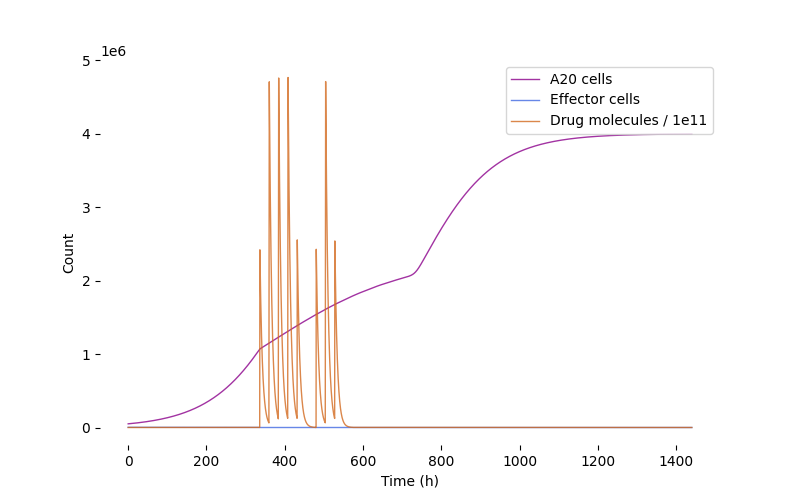
\includegraphics[scale = 0.45] {3-Ibr_high_2m.png}
    \caption{Simulation of the model with a high Ibr dose regimen}
    \label{fig:ibr-high}
\end{figure}

\begin{figure} [htbp!]
    \centering
    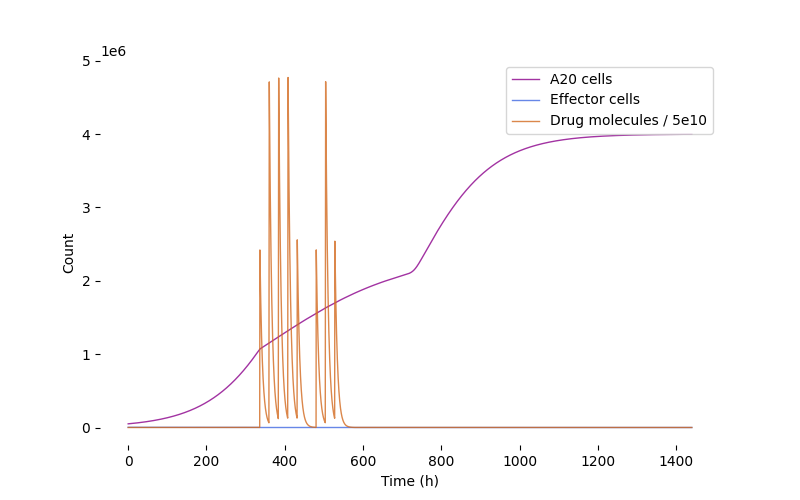
\includegraphics[scale = 0.45] {4-Ibr_low_2m.png}
    \caption{Simulation of the model with a low Ibr dose regimen}
    \label{fig:ibr-low}
\end{figure}

The dose dependency of the cytotoxicity rate $\mu_{AC}$ in the two treatment conditions with cytamidine, highlighted in \cite{main-paper}, is probably due to the 520-fold increase in drug amount of the Cyt high group with respect to the Cyt low group. The same dose dependecty is not seen in the case of Ibr, yet, in this case the increase in the drug amount is only 2-fold. Indeed, by interpolating the dose-$\mu_{AC}$ points for the two drugs, it turns out that the dose-dependecy in the efficacy of cytamidine is less that 2-fold higher that the one of ibrutinib. This can be realted to the diffeent metabolisms of the drugs.

\begin{figure} [htbp!]
    \centering
    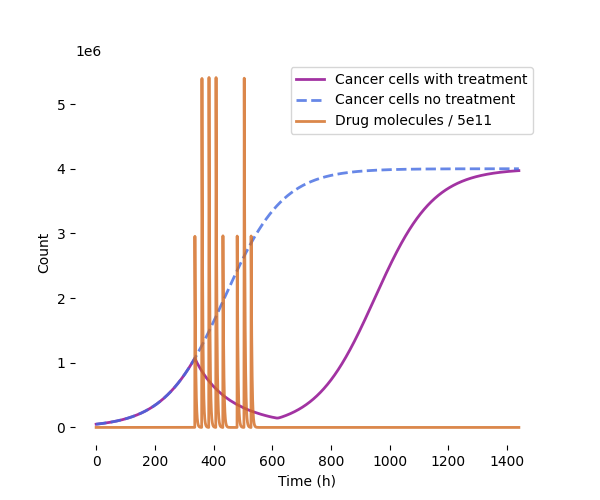
\includegraphics[scale = 0.45] {5-cyt_ibr.png}
    \caption{Simulation of the model with the absence and the presence of the combination of the two drugs}
    \label{fig:cyt-ibr}
\end{figure}

\begin{figure} [htbp!]
    \centering
    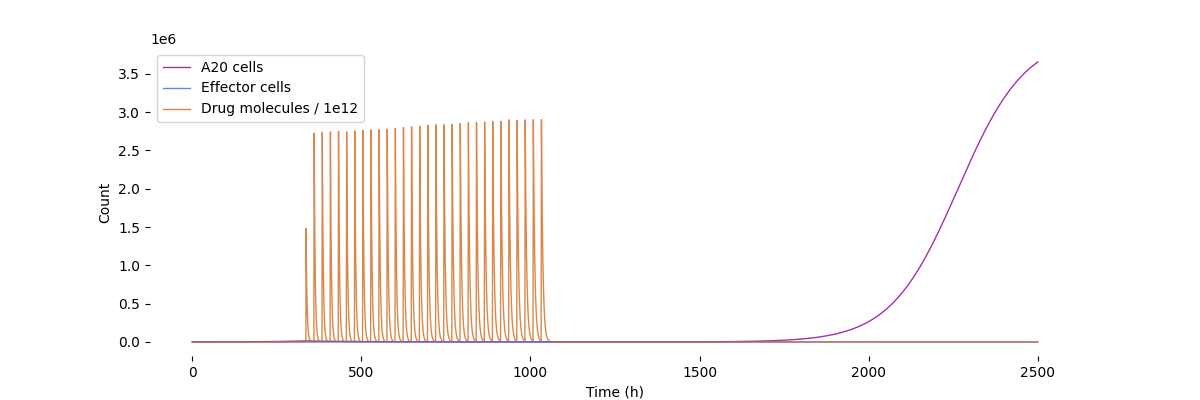
\includegraphics[scale = 0.35] {6-1e18drug.png}
    \caption{Reproduction of the Figure A2 of the main paper}
    \label{fig:1e18drug}
\end{figure}

The results of the simulations without treatments are identical to the ones reported (Figure A1 in \cite{main-paper}), and so is the growth inhibition due to the combined use of a low dose of Ibr and a high dose of Cyt for 8 days (figure 6 in \cite{main-paper} and \ref{fig:cyt-ibr}). However, there is a mismatch in what was obtained in trying to reporuce figure A2 in \cite{main-paper} and the figure itself. In particular, the most striking difference is that the tumor-free period obtained in this study due to a 30 days-long combined treatment is much shorter.\\
Regarding the adaptation of a treatment protocol involving the delivery of Cyt through infusion, the paper \cite{cyt-3}, in which Cyt is sued to threar acute myeloid leukemia in humans, was taken as referemce. Doses where adjusted according to standard guidelines \cite{dose-conversion} in order to convert them from humans to mice. It has to be noted that these treatments involved the combined use of Cyt and another drug, which parameters have not been found. Therefore, the simulations are restricted to a therapy regimen with Cyt only.
